\chapter{The Standard Model}
\label{chap:sm}

Particle physics endeavours to identify all fundamental units of matter and describe their interactions.
To this end the Standard Model (SM) of particle physics stands as the most successful theoretical framework in the history of the field.
The SM is a quantum field theory (QFT) which encompasses three out of the four fundamental forces of nature, namely the electromagnetic, weak, and strong forces.
The forth and final force, gravity, is not included in the SM\footnote{Gravity is $10^{37}$ times weaker than the weak nuclear force, and thus is negligible at the energy scales probed by particle accelerators, but can be incorporated through a coupling to a curved space-time.}.
Development of the SM was an iterative and collaborative effort that took much of the 20th century.
To date, no experimental evidence has been found to contradict the SM predictions, much to the chagrin of many physicists who are eager to find the next breakthrough.

Arguably the first major discovery in the field of particle physics was that of the electron by J.J. Thomson in 1897~\cite{ThomsonElectron}, the first elementary particle to be identified.
On the theory side, by merging the still evolving fields of quantum mechanics and special relativity, physicists Oskar Klein and Walter Gordon attempted to describe the quantum mechanical properties of relativistic electron in 1926~\cite{klein1926,Gordon1926}.
It took another two years for Paul Dirac to incorporate the spin of the electron into the theory, which also introduced the concept of  antiparticles~\cite{Dirac1928}.
The positron predicted by Dirac was observed four years later by Carl Anderson~\cite{PositiveElectron} by studying cosmic rays in cloud chambers, marking the first time a particle was discovered after being predicted theoretically.

This was closely followed by Fermi's description of $\beta$ decay~\cite{fermi1934}, which allowed for the creation and annihilation of particles, and truly solidified QFT as the correct framework for particle physics.
It also hypothesized the existence of the weak nuclear force.
More than a decade later, the method of \textit{renormalization} addressed the divergent contributions arising in perturbative QFT, a problem which had plagued the theory since its inception.
In the case of electromagnetism, the divergences were related to the self-energy of the electron and the vacuum polarization.
Using this new technique, quantum electrodynamics (QED) was fully established and with it the goal of describing the other fundamental forces of nature through renormalizable QFTs.

Starting with the discovery of the pion in 1947, a veritable explosion of new, now known to be composite, particles were discovered.
This was largely due to the development of the first particle accelerators, which for the first time allowed for the study of controlled high-energy collisions outside of cosmic rays.
Including the aforementioned pion, the kaon, lambda, and sigma particles were discovered in the late 1940s and early 1950s.
This so-called particle zoo was eventually tamed by the introduction of quarks in 1964 by Gell-Mann and Zweig~\cite{gellmann1964}.
Each of these new particles could be understood as a bound state of multiple quarks called hadrons.
Two- and three-quark states correspond to mesons and baryons, respectively.
The quark model was further solidified by the discovery of the omega-minus particle in 1964, which completed the predicted spectrum of baryons, and the discovery of the composite nature of the proton and neutron in 1968.
The theory of quarks and their interactions was formulated as a renormalizable QFT called quantum chromodynamics (QCD) in the early 1970s.

The last piece of the SM puzzle is the incorporation of the weak force via electroweak unification.
First proposed by Sheldon Glashow, this was a single QFT that combined the electromagnetic and weak forces.
While this predicted the existence of the Z-boson, it was found that the theory was non-renormalizable.
Then in 1964, the mechanism for which spontaneous symmetry breaking could lead to massive gauge bosons was developed independently by Robert Brout and François Englert, and Peter Higgs.
This was incorporated into the electroweak theory by Steven Weinberg and Abdus Salam, and the theory was shown to be renormalizable.
Experimental evidence for the electroweak theory first came in 1983 with the discovery of the W and Z bosons at CERN.
Arguably the most significant discovery in the field of particle physics was that of the Higgs boson in 2012 by the ATLAS and CMS collaborations, which at the time of writing, remains the last elementary particle to be identified.
Over 100 years after the discovery of the electron.

The SM, a combination of the electroweak and QCD theories, was developed during a time of great progress in particle physics.
This is reflected both in the advancements in the theory itself, but also in the technology and experimental techniques used to test and inform its progress.

\subsection{A Universe of Particles}

In the language of QFT, particles of both matter and force are localized excitations of corresponding quantum fields which permeate all of spacetime.
All particles are categorized by their spin segmenting the universe into two categories: spin-$\frac{1}{2}$\footnote{In units of $\hbar$} fermions and integer spin bosons.

Fermions obey Fermi-Dirac statistics and make up all physical matter in the universe.
Fermions are further divided into two subgroups: quarks and leptons.
Quarks and leptons come in three generations, each containing a charged lepton, a neutral lepton (neutrino), an \textit{up-type} quark, and a \textit{down-type} quark.
The first generation contains the lightest particles.
These include the election, electron neutrino, up quark, and down quark.
As the lightest and most stable of the three generations, these four particles make up the bulk of the matter in the universe.
The second generation contains the muon, muon neutrino, charm quark, and strange quark, and finally the third generation contains the tau, tau neutrino, top quark, and bottom quark.
Each following generation contains particles with increased mass, but otherwise identical quantum numbers to the former, and thus tend to decay into a lighter generation.
The exceptions to this rule are the neutrinos, which do not decay, but oscillate between the three generations~\cite{fukuda1998}.
Each fermion has an associated antiparticle with the same mass and spin but an opposite charge and baryon number.
A list of the fermions and their properties can be found in Table~\ref{tab:fermions}.

\begin{table}[h]
	\centering
	\caption{Fermions (spin-$\sfrac{1}{2}$ particles) of the Standard Model and their properties~\cite{ParticleDataGroup}. Not shown are the antiparticles, which have opposite charge and baryon number, but are otherwise identical.}
	\begin{adjustbox}{max width=\textwidth}
		\label{tab:fermions}
		\renewcommand{\arraystretch}{1.5}
		\begin{tabular}{c|ccc|ccc}
			\toprule
			\hline
			                        & \multicolumn{3}{c}{Leptons} & \multicolumn{3}{|c}{Quarks}                                                                 \\
			\hline
			Generation              & Flavour                     & Mass $[\MeV]$               & Charge $[e]$ & Flavour & Mass $[\MeV]$      & Charge $[e]$    \\
			\hline
			\multirow{2}{*}{First}  & e                           & 0.5110                      & -1           & $u$     & 2.16               & $+\sfrac{2}{3}$ \\
			                        & $\nu_e$                     & $< 0.8 \times 10^{-6}$      & 0            & $d$     & 4.70               & $-\sfrac{1}{3}$ \\
			\hline
			\multirow{2}{*}{Second} & $\mu$                       & 105.7                       & -1           & $c$     & $1.27 \times 10^3$ & $+\sfrac{2}{3}$ \\
			                        & $\nu_\mu$                   & $< 0.19$                    & 0            & $s$     & 93.5               & $-\sfrac{1}{3}$ \\
			\hline
			\multirow{2}{*}{Third}  & $\tau$                      & 1777                        & -1           & $t$     & $173 \times 10^3$  & $+\sfrac{2}{3}$ \\
			                        & $\nu_\tau$                  & $< 18.2$                    & 0            & $b$     & $4.18 \times 10^3$ & $-\sfrac{1}{3}$ \\
			\hline
		\end{tabular}
	\end{adjustbox}
\end{table}

Forces between fermions in a QFT manifest via the exchange of spin-1 particle called a vector- or gauge-boson.
For a fermion to interact with a given vector-boson, it must carry the corresponding charge.

In QED, the interactions are mediated by the photon and the charge is the familiar electromagnetic charge $Q$.
All fermions other than the neutrinos carry electromagnetic charge and thus couple to the photon.
The weak force is explained by the Glashow-Weinberg-Salam model (GSW)~\cite{glashow1961,weinberg1967,salam1968}, and the photon is joined by the $W^+$, $W^-$, and $Z$ bosons.
The charges of GSW theory are called \textit{weak isospin} $I$ and \textit{hypercharge} $Y$.
All fermions carry hypercharge but only left-handed fermions and right-handed antifermions carry weak isospin.
Interactions via the charged weak bosons are the only interaction which allows a change in the flavour of a fermion, e.g.\ a down-type quark can change into an up-type quark by emitting a $W^-$ boson.
Unlike the other forces in the SM, the bosons of the weak force have non-zero mass, resulting in a short range of interaction.
Finally, in QCD, particles with the \textit{colour charge} interact via the exchange of gluons.
Out of the fermions, only the quarks carry colour charge, which has three possible values labelled red, green, and blue.
Anti-quarks carry anti-colour charge, which are anti-red, anti-green, and anti-blue.
The gluons themselves carry colour charge, an eightfold combination of one colour and one anti-colour.

The last particle in the SM is the Higgs boson, which is a scalar particle with spin-0, which couples to all massive particles in the SM.
It is responsible for the generation of mass, and is the only scalar particle in the theory.
A summary of the bosons and their properties can be found in~\Cref{tab:bosons}.

\begin{table}[h]
	\centering
	\caption{Bosons (spin-1 particles) of the Standard Model and their properties~\cite{ParticleDataGroup}.
		The spin $J$ and parity $P$ of each particle are denoted by $J^P$. The strengths of the forces associated with each boson are given relative to the strong force at a distance of 1 \unit{\femto\metre}.}
	\begin{adjustbox}{max width=\textwidth}
		\label{tab:bosons}
		\renewcommand{\arraystretch}{1.5}
		\begin{tabular}{lclcccc}
			\toprule
			\hline
			Force                   & Strength                   & Boson              & Symbol   & $J^P$ & Charge $[e]$ & Mass $[\GeV]$ \\
			\hline
			Strong                  & $1$                        & Gluon              & $g$      & $1^-$ & 0            & 0             \\
			Electromagnetic         & $1^{-3}$                   & Photon             & $\gamma$ & $1^-$ & 0            & 0             \\
			\multirow{2}{*}{Weak}   & \multirow{2}{*}{$10^{-8}$} & Charged Weak boson & $W^\pm$  & $1^-$ & $\pm 1$      & $80.37$       \\
			                        &                            & Neutral Weak boson & $Z$      & $1^-$ & 0            & $91.19$       \\
			\multicolumn{2}{c}{N/A} & Higgs boson                & $H$                & $0^+$    & 0     & $125.2$                      \\
			\hline
		\end{tabular}
	\end{adjustbox}
\end{table}

\section{The Gauge Principle}
\label{sec:gauge_principle}

Symmetries have mapped out the route to most of the physical theories in this last century.
Noether's theorem famously established that continuous symmetries imply a conserved current~\cite{noether1918}.
This is often expressed through the Lagrangian formalism, where the dynamics of a system minimizes the action specified by a Lagrangian density $\mathcal{L}$.
For example, the Lagrangian of the standard model is invariant under the global Poincare group, $\text{SL}(2, \mathbb{C})$, which encompasses the symmetries of special relativity.
Under Noether's theorem, this directly leads to the conservation of energy and momentum.
Herman Weyl, a colleague of Noether, extended this to the principle of \textit{gauge theory}, a field theory where the dynamics of a system could be determined by requiring invariance under local (non-global), smooth transformations~\cite{weyl1918}.
The type of these invariances, which can be seen as belonging to a specific Lie groups, informs the interactions between the fields.
This is known as the \textit{gauge principle}.

\subsubsection{Free Field Equations}

In a QFT, all fundamental objects are described by fields which are themselves functions of spacetime $x = (t, \vec{x})$.
Observed particles are excitations of these fields.
The free (non-interacting) field Lagrangian densities describe the propagation of these fields through spacetime.

Spin-0 particles are excitations of a scalar field $\phi(x)$ such that they obey the Klein-Gordon equation,
\begin{equation}
	\label{eq:klein_gordon}
	\left( \partial_\mu \partial^\mu + m_S^2 \right) \phi = 0,
\end{equation}
where $m_S$ is the mass of the particle.
Here the index $\mu$ runs over the four dimensions of spacetime, and the Einstein summation convention is used.
This yields the Lagrangian density,
\begin{equation}
	\label{eq:scalar_lagrangian}
	\mathcal{L}_\text{S} = \frac{1}{2} \partial_\mu \phi \partial^\mu \phi - \frac{1}{2} m_S^2 \phi^2.
\end{equation}
Fermions in the standard model have spin-$\sfrac{1}{2}$ and are described by the 4-component Dirac spinor $\psi(x)$.
The equations of motions of free  fermions are described by the Dirac equation,
\begin{equation}
	\label{eq:dirac_equation}
	(i \gamma^\mu \partial_\mu - m) \psi = 0,
\end{equation}
and the Dirac Lagrangian density,
\begin{equation}
	\label{eq:dirac_lagrangian}
	\mathcal{L}_\text{Dirac} = \bar{\psi} (i \gamma^\mu \partial_\mu - m) \psi,
\end{equation}
where $\gamma^\mu(\mu=0,1,2,3)$ are the contravariant Dirac matrices\footnote{The Dirac matrices are defined by the anti-commutation relations $\{\gamma^\mu, \gamma^\nu\} = 2 g^{\mu\nu}$, where $g^{\mu\nu}$ is the Minkowski metric.}, $\bar{\psi} = \psi^\dagger \gamma^0$ is the Dirac adjoint, and $m$ is the mass of the fermion.
Finally, free spin-1 vector fields $A_\mu$ with mass $m_A$ also have a Lagrangian density given by the Proca Lagrangian,
\begin{equation}
	\label{eq:proca_lagrangian}
	\mathcal{L}_\text{Proca} = -\frac{1}{4} F_{\mu\nu} F^{\mu\nu} + \frac{1}{2} m_A^2 A_\mu^a A^{\mu},
\end{equation}
where $F_{\mu\nu}^a$ is the field strength tensor.

\subsubsection{Local Gauge Invariance}

In a gauge theory, $\mathcal{L}$ is assumed to be invariant under a set of transformations which form a Lie group $G$.
Any element of a Lie group $g \in G$ can be written as a product of exponentials of generators $g = \exp(i \theta_a T^a)$, where $\theta_a$ are the phase parameters and $T^a$ are the group generators (members of the corresponding Lie algebra).
\textit{Local gauge invariance} is expressed as phase parameters dependent on spacetime, $\theta_a(x)$.
The Lagrangian is therefore required to be invariant under some transformation $\psi \rightarrow \exp\left(i \theta_a(x) T^a\right) \psi$.

Taking the Dirac Lagrangian density as an example, it is clear that $L_\text{Dirac}$ is not invariant under local phase transformations.
To remedy this, the covariant derivative $D_\mu$ is introduced,
\begin{equation}
	\label{eq:covariant_derivative}
	D_\mu = \partial_\mu - i g T^a A_\mu^a,
\end{equation}
where $A_\mu^a$ represents a spin-1 vector field for each generator and $g$ is some scalar labelled the \textit{coupling constant}.
The field itself is required to transform as,
\begin{equation}
	\label{eq:gauge_transformation}
	A_\mu^a \rightarrow A_\mu^a - g^{-1} \partial_\mu \theta^a - f^{abc} \theta^b A_\mu^c,
\end{equation}
where $f^{abc}$ are the \textit{structure constants} of $G$ given given by the relation,
\begin{equation}
	\label{eq:structure_constants}
	[T^a, T^b] = i f^{abc} T^c.
\end{equation}
The term on the left denotes the commutator Lie bracket $[A, B] = AB - BA$.
In an Abelian group, the structure constants are all trivially zero.
Inserting the covariant derivative into the Dirac Lagrangian density yields,
\begin{align}
	\label{eq:dirac_lagrangian_gauge}
	\mathcal{L_D} & = \bar \psi (i \gamma^\mu D_\mu - m) \psi                                                                                                                                       \\
	              & = \underbrace{\bar \psi (i \gamma^\mu \partial_\mu - m) \psi}_\text{free spinor} \quad + \quad \underbrace{g \bar \psi \gamma^\mu A_\mu^a \psi}_\text{\shortstack{spinor-vector \\interaction}}.
\end{align}
This modified Dirac Lagrangian no longer describes a free fermion field $\psi$ but one that interacts with a vector field $A_\mu^a$ with strength $g$.

The existence $A_\mu^a$ also means that it should contribute to the Lagrangian density of the system via the Proca Lagrangian.
Expanding out the field strength tensor (generalized to non-Abelian groups) gives,
\begin{equation}
	\label{eq:field_strength_tensor}
	F_{\mu\nu}^a = \partial_\mu A_\nu^a - \partial_\nu A_\mu^a - g f^{abc} A_\mu^b A_\nu^c
\end{equation}
The Proca Lagrangian is therfore be expanded to give,
\begin{align}
	\label{eq:boson}
	\mathcal{L}_\text{Proca} =
	 & -\frac{1}{4}(\partial_\mu A_\nu^a - \partial_\nu A_\mu^a) (\partial^\mu A^{a\nu} - \partial^\nu A^{a\mu}) &  & \leftarrow \text{dynamics}            \\
	 & + \frac{1}{2} g f^{abc} (\partial_\mu A_\nu^a - \partial_\nu A_\mu^a) A^{b\mu} A^{c\nu}                   &  & \leftarrow \text{triple interaction}  \\
	 & - \frac{1}{2} g^2 f^{abc} f^{ade} A_\mu^b A_\nu^c A^{d\mu} A^{e\nu}                                       &  & \leftarrow \text{quartic interaction} \\
	 & + \frac{1}{2} \cancelto{0}{m_A^2} A_\mu^a A^{a\mu}                                                        &  & \leftarrow \text{mass term}.
\end{align}
The first thing to note is that the mass term for the vector boson has been cancelled out.
This is because the quadratic $A_\mu^a A^{a\mu}$ is not invariant under the transformation in \Cref{eq:gauge_transformation}, leading to the conclusion that either the vector boson is massless or that the symmetry is broken in some way.
The terms derived from the field strength tensor $F_{\mu\nu}^a F^{a\mu\nu}$ are trivially invariant under the local gauge transformation.
In the non-Abelian case (non-zero structure constants), the Lagrangian includes additional interaction terms with the field and itself.
These are called triple and quartic \textit{self-couplings}.

The necessity for local gauge invariance of a theory describing fermions suggests the presence of a new massless gauge field characterized by specific gauge transformation properties.
Each of the generators of the group also correspond to a hermitian operator acting on the field, which can be interpreted as the charge of the particle.
The full Lagrangian for the system $\mathcal{L} = \mathcal{L}_D + \mathcal{L}_\text{Proca}$ contains terms for the free fermion field, interactions between fermion field and the gauge fields, and self-interactions terms of the gauge fields if the group is non-Abelian.

\section{Symmetries of the Standard Model}
\label{sec:symmetries_of_sm}

The Lie group of local gauge transformations observed by the SM Lagrangian can be expressed as the product of three simple groups,
\begin{equation}
	\label{eq:sm_group}
	\text{SU}(3)_C \times \text{SU}(2)_L \times \text{U}(1)_Y.
\end{equation}
Here the subscripts $C$ and $L$ denote the colour and left-handedness of the fermions, respectively, and $Y$ is the hypercharge.
Adherence to $\text{SU}(3)_C$ gives rise to interactions via the strong force, which is described by QCD\@ and outlined in \Cref{sec:qcd}.
The $\text{SU}(2)_L \times \text{U}(1)_Y$ group corresponds to the unified electroweak force, which is described in \Cref{sec:electroweak}.
Each force has a corresponding charge which is conserved interactions.

The Lagrangian of the SM can be given by,
\begin{equation}
	\label{eq:sm_lagrangian}
	\mathcal{L}_\text{SM} = i \bar \psi \gamma^\mu D_\mu \psi -\frac{1}{4} F_{\mu\nu} F^{\mu\nu} + (y_{ij} \bar \psi_i \phi \psi_j + \text{h.c.}) + |D_\mu \phi|^2 - V(\phi).
\end{equation}
The first term refers to the fermions and their interactions with the gauge bosons.
The second term refers to gauge bosons and their self couplings.
Conspicuously absent is the mass term for the fermions.
This is because mass in the SM is generated via the Higgs mechanism, which  introduces a new scalar (spin-0) field $\phi$ and the final three terms in \Cref{eq:sm_lagrangian}, namely the Yukawa couplings, the Higgs interaction with the vector bosons, and the Higgs potential respectively.
The h.c.\ in the Yukawa term denotes the Hermitian conjugate.
The Higgs mechanism described in \Cref{sec:higgs}.

\subsection{U(1) \texorpdfstring{$\rightarrow$}{-} Quantum Electrodynamics}

QED provides a simple example of the gauge principle in action.
All gauge theories start with the assumption of a local symmetry that the universe adheres to and the simplest of these is the $\text{U}(1)$ symmetry of electromagnetism.
This is expressed as $\psi \rightarrow \hat U(x) \psi$, where $\hat U(x) = \exp{i Q \chi(x)}$ for some arbitrary scalar field $\chi(x)$ and coupling strength (particle charge) $Q$.
Applying this transformation to the free Dirac Lagrangian density results in an imbalance,
\begin{align}
	i \gamma^\mu \partial_\mu ( e^{i Q \chi} \psi ) - m e^{i Q \chi}  \psi                                          & = 0                                      \\
	e^{i Q \chi} i \gamma^\mu \left[ \partial_\mu \psi + i Q (\partial_\mu \chi) \psi \right] - m e^{i Q \chi} \psi & = 0                                      \\
	(i \gamma^\mu \partial_\mu - m) \psi                                                                            & = Q \gamma^\mu (\partial_\mu \chi) \psi.
	\label{eq:imbalanced_dirac}
\end{align}
For the equation to remain invariant under the local phase transformation, the right-hand side of \Cref{eq:imbalanced_dirac} must vanish.
Following the procedure in \Cref{eq:gauge_transformation}, a new field $A_\mu$ is introduced, transforming as,
\begin{equation}
	\label{eq:photon_transformation}
	A_\mu \rightarrow A_\mu - \partial_\mu \chi.
\end{equation}
The covariant interaction term between is therefore given by,
\begin{equation}
	\label{eq:qed_interaction}
	Q \gamma ^\mu A_\mu \psi \rightarrow Q \gamma^\mu A_\mu \psi e^{i Q \chi} + Q \gamma^\mu (\partial_\mu \chi) \psi e^{i Q \chi},
\end{equation}
which cancels out the right-hand side of \Cref{eq:imbalanced_dirac}.

As $\text{U}(1)$ is Abelian, the structure constants disappear and the vector field does not self-interact.
This results in the QED Lagrangian density,
\begin{align}
	\mathcal{L}_\text{QED} & = \overbrace{-\frac{1}{4} F_{\mu\nu} F^{\mu\nu}}^{\text{free photon}} + \overbrace{\bar \psi (i \gamma^\mu \partial_\mu - m) \psi}^{\text{free fermion}} + \overbrace{Q \bar \psi \gamma^\mu A_\mu \psi}^{\text{interaction}} \\
	                       & = -\frac{1}{4} F_{\mu\nu} F^{\mu\nu} + \bar \psi (i \gamma^\mu D_\mu - m) \psi.
	\label{eq:qed_lagrangian}
\end{align}
Note that the interaction term is absorbed into the covariant derivative in \Cref{eq:qed_lagrangian}.

Therefore, by the simple requirement that physics is invariant under a local $\text{U}(1)$ transformation, an interaction between the fermion field and a massless spin-1 field, now known to be the photon field, is required.
The strength of these interactions being proportional to the charge of the particle.
In the SM, $\mathcal{L}_\text{QED}$ is combined into the electroweak Lagrangian density, described in \Cref{sec:electroweak}.

\subsection{\texorpdfstring{$\text{SU(3)}_C\rightarrow$}{SU(3)-} Quantum Chromodynamics}
\label{sec:qcd}

The strong force is described by the gauge theory of QCD, which is based on the $\text{SU}(3)_C$ symmetry group.
This is an eight-dimensional group often expressed by all $3 \times 3$ unitary matrices with determinant 1.
The eight generators of the group $T^a{ }(a = 1, \ldots, 8)$ are typically expressed as $T^a = \sfrac{\lambda^a}{2}$, where $\lambda^a$ are the Gell-Mann matrices~\cite{gellmannmatrices}.
The phase parameter $\theta^a(x)$ also represents eight functions of spacetime.
The fermion spinor $\psi$ acquires a new index representing three new degrees of freedom called \textit{color}.

The group is non-Abelian, making it a Yang-Mills theory \cite{yangmills}, and the non-zero structure constants are given by,
\begin{equation}
	\label{eq:qcd_sc}
	\begin{array}{ccc}
		f_{123} = 1 ,                                                            & \hspace{\stretch{1}}
		f_{147} = f_{516} = f_{246} = f_{257} = f_{345} = f_{637} = \frac{1}{2}, & \hspace{\stretch{1}}
		f_{458} = f_{678} = -\frac{1}{2}.
	\end{array}
\end{equation}
Following the standard procedure outlined in \Cref{sec:gauge_principle} the covariant derivative is given by,
\begin{equation}
	\label{eq:qcd_covariant_derivative}
	D_\mu = \partial_\mu - i g_s T^a G_\mu^a,
\end{equation}
where $G_\mu^a$ represents eight gluon fields and $g_s$ is the strong coupling constant.
The transformation properties of the gluon fields are given by \Cref{eq:gauge_transformation}, and the field strength tensor is given by \Cref{eq:field_strength_tensor}.
The QCD Lagrangian density, in terms of the coloured component of the fermion field $q_i(i = 1, 2, 3)$ is,
\begin{equation}
	\label{eq:qcd_lagrangian}
	\mathcal{L}_\text{QCD} = -\frac{1}{4} G_{\mu\nu}^a G^{a\mu\nu} + \bar q_i (i \gamma^\mu D_\mu - m) q_i.
\end{equation}

The scattering amplitudes in a QFT is calculated via the perturbative expansion of interaction terms in the Lagrangian using a Dyson series.
Infinities arising in the expansion are removed by a process called renormalization, which introduces a dependence on the energy scale of the interaction for the effective coupling constants.
For the electromagnetic and weak forces the coupling strength increases with the momentum transfer of the interaction, but this dependence is minor.
For the strong force the coupling constant becomes significantly weaker as the energy scale increases and the length scale decreases.
This is a phenomenon known as \textit{asymptotic freedom}~\cite{gross1973} and is shown in \Cref{fig:asymptotic_freedom}.
At the high energies of collider experiments ($ > 100 \GeV$), the quarks, even though bound in hadrons, behave as free particles.
Conversely, at low energies the coupling constant becomes close to unity.
\begin{figure}[h]
	\centering
	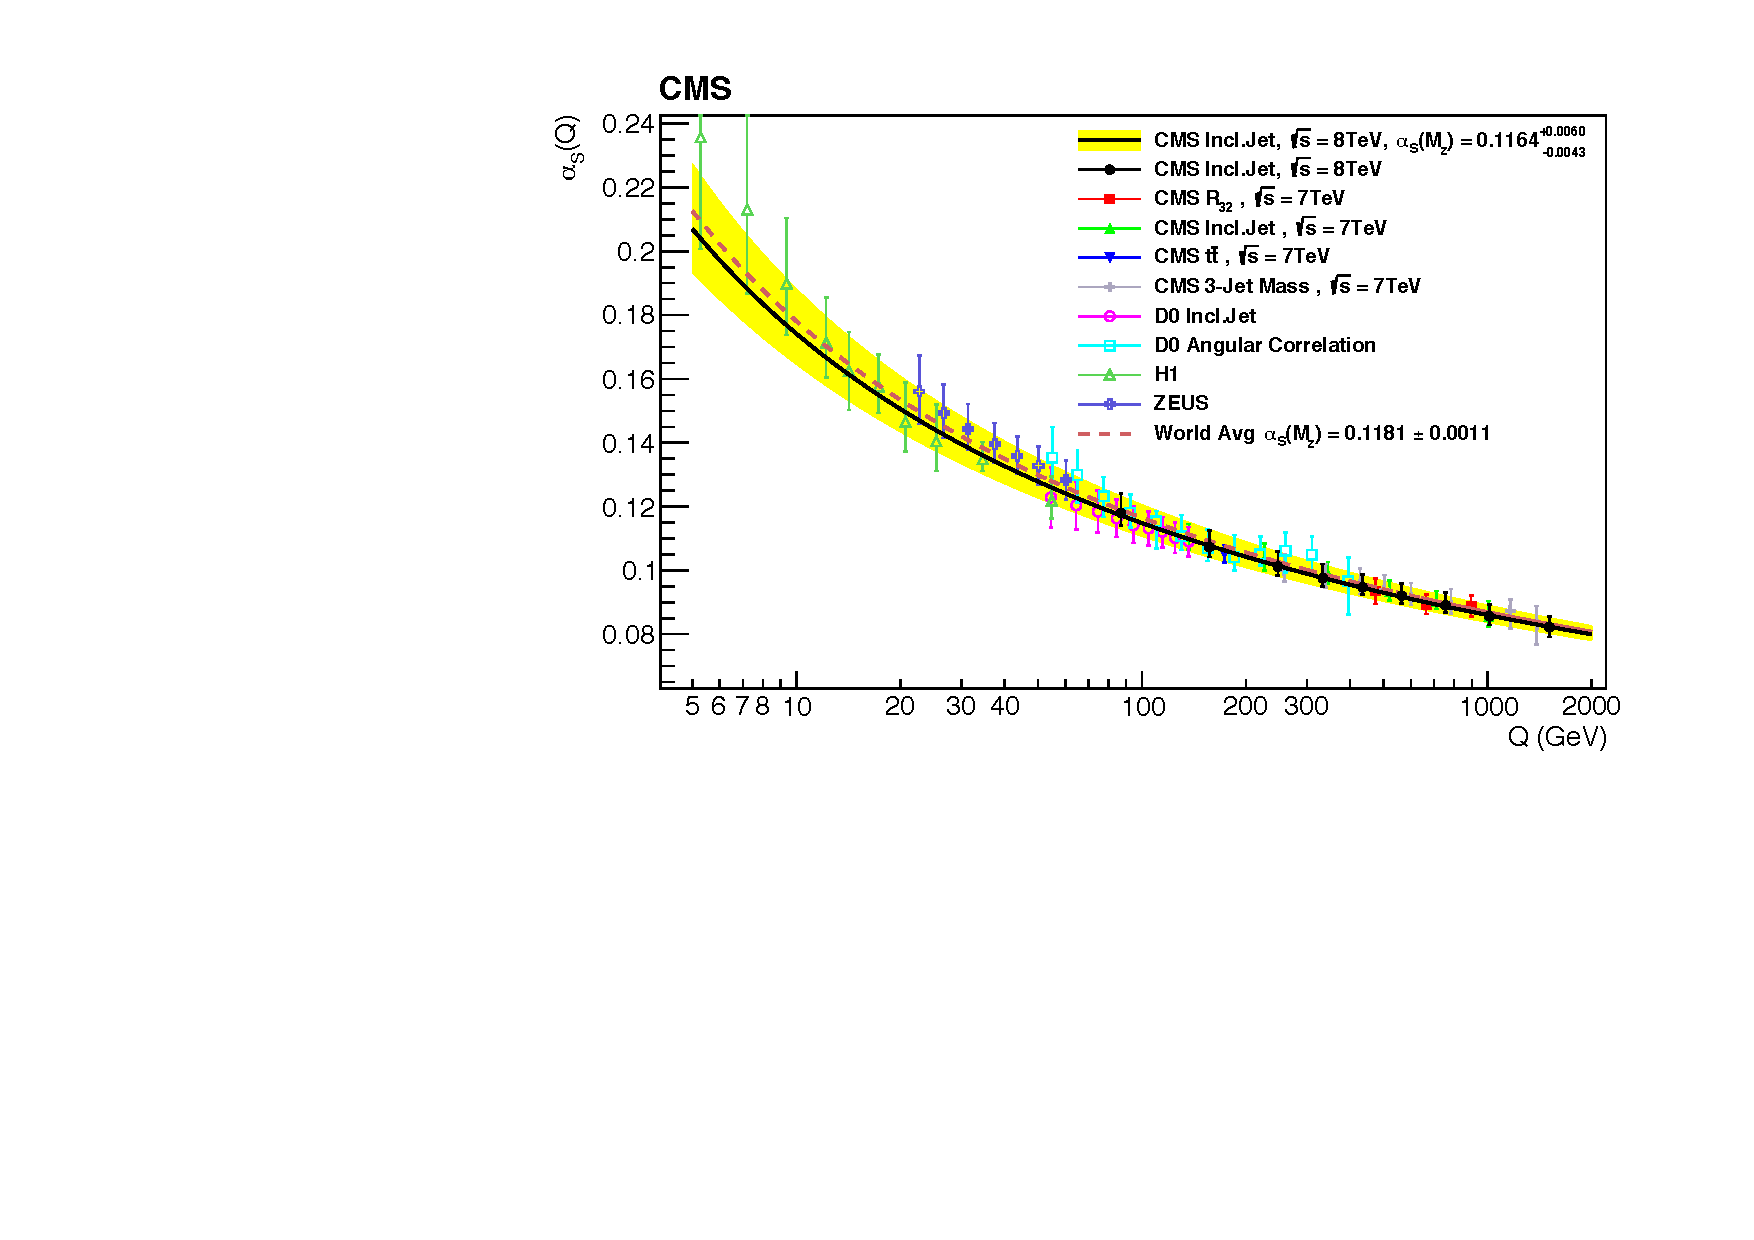
\includegraphics[width=0.7\textwidth]{Figures/standard_model/running}
	\caption{The running of the strong coupling constant $\alpha_s = \sfrac{g_s^2}{4\pi}$ as a function of the energy scale $Q$ as measured by experiments at the LHC, Tevatron, and HERA~\cite{CMSRunning}.}
	\label{fig:asymptotic_freedom}
\end{figure}
At these scales divergences are induced and the theory can't be treated perturbatively.
An observed effect at this scale is \textit{color confinement} where quarks and gluons are never isolated, but are always bound together in color-neutral ($\text{SU}(3)$ invariant) states called hadrons.
A consequence of confinement is hadronisation, the process by which high energy colored particles form particle jets, which is described in \Cref{sec:jets}.
As the theory is non-perturbative, there is no analytical description for confinement.

\subsection{\texorpdfstring{$\text{SU}(2)_L \times \text{U}(1)_Y \rightarrow$}{SU(2)xSU(1)-} Electroweak Theory}
\label{sec:electroweak}

In the electroweak model of Glashow, Salam, and Weinberg (QSW), QED and the weak force are unified into a single theory and a combined group $\text{SU}(2)_L \times \text{U}(1)_Y$.
As with all gauge theories, this introduces four gauge fields corresponding to each generator of the group.
\begin{align}
	\text{SU}(2)_L & \rightarrow W_\mu^a(a = 1, 2, 3) \\
	\text{U}(1)_Y  & \rightarrow B_\mu
\end{align}
The $\text{SU}(2)_L$ group is non-Abelian making this a Yang-Mills theory, and the structure constants are given by $f^{abc} = \epsilon^{abc}$, where $\epsilon^{abc}$ is the Levi-Civita symbol.
The generators of the group are the based on the three Pauli spin matrices $\sigma^i$~\cite{paulispin}.
\begin{equation}
	\label{eq:su2_generators}
	T^a \equiv I^a = \frac{\sigma^a}{2} \\
\end{equation}
\begin{equation}
	\sigma^1 = \begin{pmatrix} 0 & 1 \\ 1 & 0 \end{pmatrix},
	\quad \sigma^2 = \begin{pmatrix} 0 & -i \\ i & 0 \end{pmatrix},
	\quad \sigma^3 = \begin{pmatrix} 1 & 0 \\ 0 & -1 \end{pmatrix}.
	\label{eq:pauli_matrices}
\end{equation}
The strength tensors are given by
\begin{align}
	\label{eq:ew_field_strength_tensors}
	W_{\mu\nu}^a & = \partial_\mu W_\nu^a - \partial_\nu W_\mu^a - g \epsilon^{abc} W_\mu^b W_\nu^c, \\
	B_{\mu\nu}   & = \partial_\mu B_\nu - \partial_\nu B_\mu.
\end{align}
It is useful to split the fermion fields into left- and right-handed components using chiral the projection operators $P_{L/R} = \sfrac{1}{2} (1 \mp \gamma^5)$, where $\gamma^5 = i \gamma^0 \gamma^1 \gamma^2 \gamma^3$.
Experimentally, the charged weak current has proved to be maximally parity violating.
This means that the interaction term must follow a V-A (vector-axial) coupling type which can be shown to be equivalent to a standard coupling to left-handed fermions only:
\begin{equation}
	\label{eq:v-a_coupling}
	\mathcal{L}_\text{V-A}
	= \frac{1}{2} \bar \psi \gamma^\mu (1 - \gamma^5) \psi W_\mu
	= \bar \psi \gamma^\mu P_L \psi W_\mu
	= \bar \psi P_R \gamma^\mu P_L \psi W_\mu
	= \bar \psi_L \gamma^\mu \psi_L W_\mu.
\end{equation}
Therefore only left-handed fermions (and right-handed antifermions) carry non-zero weak isospin.
The covariant derivative is given by,
\begin{equation}
	\label{eq:ew_covariant_derivative}
	D_\mu = \partial_\mu - i g_W \frac{\sigma_a}{2} W_\mu^a - i g_Y \frac{Y}{2} B_\mu,
\end{equation}
where $g_W$ and $g_Y$ are the weak and hypercharge coupling constants respectively.
The Lagrangian for electroweak theory is,
\begin{align}
	\begin{split}
		\label{eq:ew_lagrangian}
		\mathcal{L}_\text{EW} = & - \bar{\psi}_L \left( \gamma^\mu g_W \frac{1}{2} \sigma^a W^a_\mu + \gamma^\mu g_Y \frac{Y}{2} B_\mu \right) \psi_L - \bar{\psi}_R \left( \gamma^\mu g_Y \frac{Y}{2} B_\mu \right) \psi_R \\
		                        & - \frac{1}{4} W_{\mu\nu}^a W^{a\mu\nu} - \frac{1}{4} B_{\mu\nu} B^{\mu\nu}.
	\end{split}
\end{align}
As a Yang-Mills theory, the gauge fields $W_\mu^a$ interact in quadratic and triple self-couplings.

The $2 \times 2$ Pauli matrices require two new components to the fermion wave function which are described as weak isospin doubles.
The left-handed fermions (and right-handed antifermions)
are placed in doublets which differ by a unit of charge.
Up-type quarks and neutrinos have a weak isospin of $\sfrac{1}{2}$, while down-type quarks and charged leptons have a weak isospin of $-\sfrac{1}{2}$.
The corresponding weak eigenstate doublets are given by,
\begin{equation}
	\label{eq:weak_isospin}
	\begin{pmatrix} \nu_e \\ e \end{pmatrix}_L,
	\begin{pmatrix} \nu_\mu \\ \mu \end{pmatrix}_L,
	\begin{pmatrix} \nu_\tau \\ \tau \end{pmatrix}_L,
	\begin{pmatrix} u \\ d' \end{pmatrix}_L,
	\begin{pmatrix} c \\ s' \end{pmatrix}_L,
	\begin{pmatrix} t \\ b' \end{pmatrix}_L.
\end{equation}
The right-handed fermions (and left-handed antifermions) do not carry isospin and are placed in singlets.
The effect of the charged weak interaction is therefore to rotate these doublets, effectively changing the flavour of the fermion\footnote{Since there is no other force through which the neutrinos can interact, there are no right-handed neutrinos in the SM.}.

The isospin doublets are described with respect to the weak eigenstates, which do not correspond to the observable mass eigenstates.
The down-type quarks by convention mix between the weak eigenstates ($d', s', b'$) and the mass eigenstates ($d, s, b$) through the CKM matrix~\cite{cabibbo1963},
\begin{equation}
	\label{eq:ckm_matrix}
	\begin{pmatrix} d' \\ s' \\ b' \end{pmatrix} =
	\begin{pmatrix} V_{ud} & V_{us} & V_{ub} \\ V_{cd} & V_{cs} & V_{cb} \\ V_{td} & V_{ts} & V_{tb} \end{pmatrix} \begin{pmatrix} d \\ s \\ b \end{pmatrix} =
	\begin{pmatrix} 0.974 & 0.224 & 0.004 \\ 0.221 & 0.975 & 0.041 \\ 0.009 & 0.042 & 1.014 \end{pmatrix} \begin{pmatrix} d \\ s \\ b \end{pmatrix},
\end{equation}
where the numerical values of the elements are determined experimentally~\cite{ParticleDataGroup}\footnote{The non-unitary nature of experimental values of the CKM matrix is in tension with the SM by 2.2$\sigma$}.
For the leptons, the mixing is described with respect to the neutrinos and the PMNS matrix~\cite{pontecorvo1967, maki1962}.
These matrices provide explanations for the observed neutrino oscillations and the CP violation of the weak sector.

\subsection{Electroweak Symmetry Breaking}
\label{sec:higgs}

GSW theory predicts 4 gauge fields $W^a_\mu$ and $B_\mu$ which do not correspond to the physical $W^\pm$, $Z$, and $\gamma$ bosons.
As a requirement of gauge invariance these fields are deemed to be massless, which is also in contradiction with the observed massive $W^\pm$ and $Z$ bosons.
These discrepancies are resolved by the Brout-Englert-Higgs mechanism~\cite{higgs1964, englert1964, brout1964} (referred to hereafter as the Higgs mechanism), and the spontaneous symmetry breaking of the electroweak symmetry group (EWSB).
Spontaneous symmetry breaking is a phenomenon where the ground state of a system does not exhibit the same symmetries of the Lagrangian.

Consider a new scalar field given by a complex doublet,
\begin{equation}
	\phi = \begin{pmatrix} \phi^+ \\ \phi^0 \end{pmatrix} = \frac{1}{\sqrt{2}} \begin{pmatrix} \phi_1 + i \phi_2 \\ \phi_3 + i \phi_4 \end{pmatrix},
\end{equation}
embedded in a theory which observes the local $\text{SU}(2)_L \times \text{U}(1)_Y$ symmetry of the GSW model.
The Lagrangian density for the free scalar field, defined with the same covariant derivatives of \Cref{eq:ew_covariant_derivative}, is given by,
\begin{equation}
	\label{eq:higgs_lagrangian}
	\mathcal{L} = (D_\mu \phi)^\dagger (D^\mu \phi) - V(\phi).
\end{equation}
Here, $V(\phi)$ is a potential term describing the field self-interactions.
The specific potential encountered in the Higgs mechanism is defined as,
\begin{equation}
	\label{eq:higgs_potential}
	V(\phi) = \mu^2 \phi^\dagger \phi + \lambda (\phi^\dagger \phi)^2,
\end{equation}
where $\mu^2$ and $\lambda$ are free parameters of the theory with some restrictions.
The value of $\lambda$ is required to be positive to ensure the potential is bounded from below, allowing a stable vacuum state (the state of lowest energy).
The value of $\mu^2$ is constrained to be negative to allow for spontaneous symmetry breaking.
The vacuum state is found by minimising the Hamiltonian of the system corresponds to a constant scalar field satisfying,
\begin{equation}
	\frac{\partial V}{\partial \phi} = 0 \Longrightarrow  \phi^\dagger \phi = -\frac{\mu^2}{2\lambda} \equiv \frac{v^2}{2},
\end{equation}
where $v$ is the vacuum expectation value of the field.

\begin{figure}[h]
	\centering
	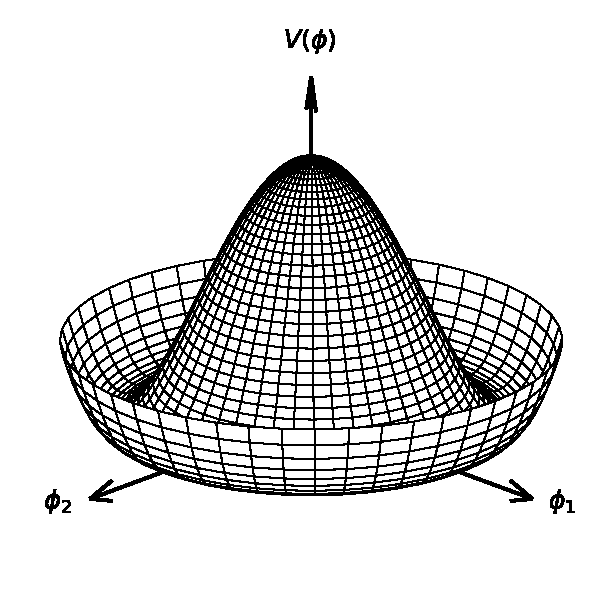
\includegraphics[width=0.5\textwidth]{Figures/standard_model/mexican_hat_potential}
	\caption{The form of the Higg's potential $V(\phi)$ if $\mu^2 < 0$ and $\lambda > 0$ respect to the first component of the complex doublet}
	\label{fig:mexican_hat}
\end{figure}

As shown in \Cref{fig:mexican_hat}, the potential has an infinite number of vacuum states satisfying this condition.
Physically, the vacuum will fall into one of these states, spontaneously breaking the symmetry of the Lagrangian.
With no loss of generality, the physical vacuum state is chosen to be,
\begin{equation}
	\label{eq:higgs_vacuum}
	| 0 \rangle	= \frac{1}{\sqrt{2}} \begin{pmatrix} 0 \\ v \end{pmatrix}.
\end{equation}
In order to use perturbation theory, the field $\phi$ is expanded about the vacuum state $|0\rangle$,
\begin{equation}
	\phi(x) = \frac{1}{\sqrt{2}} \begin{pmatrix} \phi_1(x) + i \phi_2(x) \\ v + \phi_3 + i \phi_4(x) \end{pmatrix}.
\end{equation}

The expected form of the symmetry breaking should result in the group of QED,
\begin{equation}
	\text{SU}(2)_L \times \text{U}(1)_Y \rightarrow_\text{EWSB} \text{U}(1)_\text{Q},
\end{equation}
where $Q$ refers to the electric charge.
The Goldstone theorem states that for every spontaneously broken continuous symmetry, there exists a massless scalar boson; one for each generator of the group.
In EWSB, the broken symmetry should result in three massless Goldstone bosons, however there is no experimental evidence for such massless scalar particles.
The Higgs mechanism resolves this by absorbing the Goldstone bosons through an appropriate selection of gauge.
It's crucial to note that physical predictions remain unchanged regardless of the gauge, but by selecting the \textit{unitary gauge}, the Goldstone bosons vanish, and the fields in the Lagrangian represent the actual physical particles.
In the unitary gauge the scalar field is given by,
\begin{equation}
	\label{eq:higgs_unitary_gauge}
	\phi(x) = \frac{1}{\sqrt{2}} \begin{pmatrix} 0 \\ v + h(x) \end{pmatrix},
\end{equation}
where $h(x)$ is the physical massive Higgs field, the excitation of which is the Higgs boson $H$.

The relationship between weak isospin, hypercharge, and electric charge is given by,
\begin{equation}
	\label{eq:hypercharge}
	Q = I^3 + \frac{Y}{2}.
\end{equation}
As the only surviving massless boson is the photon, $\text{U}(1)_\text{Q}$ must remain a symmetry of the vacuum state.
This is achieved by setting the electric charge of the vacuum state to zero, or equivalently $Y=1$.
Using the definitions from \Cref{eq:pauli_matrices} and \Cref{eq:ew_covariant_derivative} the covariant derivative is given by
\begin{equation}
	\label{eq:higgs_covariant_derivative}
	D_\mu = \frac{1}{2}
	\begin{pmatrix}
		2 \partial_\mu + i g_W W_\mu^3 + i g_Y B_\mu &
		i g_W (W_\mu^1 - i W_\mu^2)                    \\
		i g_W (W_\mu^1 + i W_\mu^2)                  &
		2 \partial_\mu - i g_W W_\mu^3 + i g_Y B_\mu
	\end{pmatrix}
\end{equation}
Combining this with the unitary gauge scalar field yields the first term of the Higgs Lagrangian,
\begin{align}
	\label{eq:higgs_lagrangian_1}
	\begin{split}
		(D_\mu \phi)^\dagger (D^\mu \phi) =
		\frac{1}{2} \partial_\mu h \partial^\mu h
		+ \frac{1}{8} g_W^2 (W_\mu^1 + i W_\mu^2)(W^{1\mu} - i W^{2\mu})(v + h)^2
		\\
		+ \frac{1}{8} (g_W W_\mu^3 - g_Y B_\mu)(g_W W^{3\mu} - g_Y B^\mu)(v + h)^2.
	\end{split}
\end{align}
One can identify the massive physical fields by the terms in \Cref{eq:higgs_lagrangian_1} that are quadratic in the gauge boson fields and do not contain the Higgs field.
\begin{equation}
	W^\pm_\mu = \frac{W^1_\mu \mp i W^2_\mu}{\sqrt{2}}
	\qquad
	Z_\mu = \frac{g_W W^3_\mu - g_Y B_\mu}{\sqrt{g_W^2 + g_Y^2}}
	\qquad
	A_\mu = \frac{g_W B_\mu + g_Y W^3_\mu}{\sqrt{g_W^2 + g_Y^2}}.
\end{equation}
Rewriting out \Cref{eq:higgs_lagrangian} in terms of the physical fields and in the unitary gauge gives,
\begin{equation}
	\label{eq:higgs_lagrangian_full}
	\resizebox{.99\hsize}{!}{$
			\begin{aligned}
				\mathcal{L}_{EW+H}
				 & = \underbrace{\vphantom{\frac{}{}} - \lambda v^2 h^2}_{H \text{ mass}}
				\underbrace{+\frac{1}{4} g_W^2 v^2 W^-_\mu W^{+\mu}}_{W \text{ mass}}
				\underbrace{+\frac{1}{8} g_Y^2 v^2 Z_\mu Z^\mu}_{Z \text{ mass}}                                                                                 \\
				 & \underbrace{+\frac{1}{2} g_W^2 v h W^-_\mu W^{+\mu}}_{HWW}
				\underbrace{+\frac{1}{4} g_W^2 h^2 W^-_\mu W^{+\mu}}_{HHWW}
				\underbrace{+\frac{1}{4} g_Y^2 v h Z_\mu Z^\mu}_{HZZ}
				\underbrace{+\frac{1}{8} g_Y^2 h^2 Z_\mu Z^\mu}_{HHZZ}                                                                                           \\
				 & \underbrace{+\frac{1}{2}(\partial_{\mu} h)(\partial^{\mu} h) - \lambda v h^3 + \frac{1}{4}\lambda h^4}_{h\text{ dynamics and self-couplings}}
				\underbrace{+\frac{1}{4} W^a_{\mu\nu} W^{a\mu\nu} + \frac{1}{4} B_{\mu\nu} B^{\mu\nu}}_{\text{EW dynamics and self-couplings}}.
			\end{aligned}
		$}
\end{equation}
From the top row of \Cref{eq:higgs_lagrangian_full} the masses of each of the bosons can be identified,
\begin{equation}
	\label{eq:ew_masses}
	m_W = \frac{1}{2} g_W v
	\qquad
	m_Z = \frac{1}{2} v \sqrt{g_W^2 + g_Y^2}
	\qquad
	m_A = 0
	\quad
	m_H = \sqrt{2 \lambda} v.
\end{equation}
The bottom row of \Cref{eq:higgs_lagrangian_full} includes the dynamics and self-couplings of the electroweak fields in their original form before EWSB due to convenience.
Expanding this term with respect to the physical fields results in trilinear interactions between the photon and the $W^\pm$ bosons.
The free parameters of the GSW + Higgs mechanism are the electroweak coupling constants $g_W$ and $g_Y$, the Higgs self-coupling $\lambda$, and the vacuum expectation value $v$, all of which are determined experimentally.

The final piece of the SM is the generation of fermion masses through the Higgs mechanism.
Due to the different transformation properties of the left- and right-handed fermions, the standard mass term $m \bar \psi \psi$ mixes the left- and right-handed components and thus is not invariant under the electroweak symmetry group.
The Yukawa interaction term is introduced to couple each of the fermions doublets to the Higgs field.
For example the electron mass term is given by,
\begin{equation}
	\label{eq:yukawa}
	\begin{split}
		\mathcal{L}_\text{Yukawa} & = -g_e( \bar \psi_L \phi \psi_R + \bar \psi_R \phi^\dagger \psi_L)    \\
		                          & = -g_e \left[
			\begin{pmatrix} \bar \nu_e & \bar e \end{pmatrix}_L \begin{pmatrix} 0 \\ \frac{v + h}{\sqrt{2}} \end{pmatrix} e_R
			+ \bar e_R \begin{pmatrix} 0 & \frac{v + h}{\sqrt{2}} \end{pmatrix} \begin{pmatrix} \nu_e \\ e \end{pmatrix}_L
		\right]                                                                                           \\
		                          & = -\frac{g_e v}{\sqrt{2}} \bar e e - \frac{g_e}{\sqrt{2}} \bar e e h,
	\end{split}
\end{equation}
where $g_e$ is the electron Yukawa coupling constant.
A similar prescription can be applied other leptons, the up-type, and down-type quarks to yield the relationship of the fermion masses $m_f$ to the Yukawa coupling constants $g_f$ and the Higgs vacuum expectation value,
\begin{equation}
	\label{eq:fermion_mass}
	m_f = \frac{g_f v}{\sqrt{2}}.
\end{equation}

\section{Particle Jets}
\label{sec:jets}

